\chapter{Testing}
Testing is an important aspect of the work carried out in this thesis. In this chapter the
test setup are described. How the tests are carried out, some of the results and some
immediate results.


\section{Test Environment}
The test environment are two connected pipe segments. A Y-junction and an L-bend. This
pipe segments are connected, according to Figure \ref{chap7:fig-environment}.

\begin{figure}[htbp]
    \centering
  %  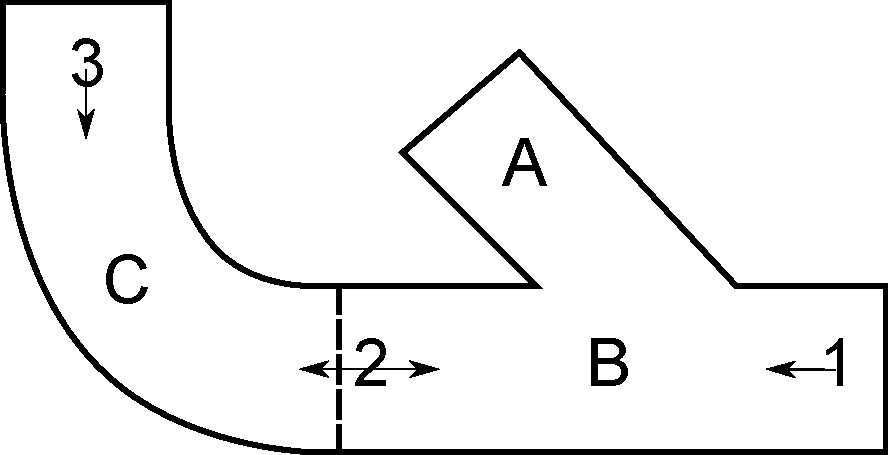
\includegraphics[width=0.7\textwidth]{pics/test-environment}
    \caption{The test environment}
    \label{chap7:fig-environment}
\end{figure}

There are six points of interest in this environment. 
The numbers 1-3 are the places where the sensors will be put and record snapshots of the pipe. 
The letters A-C are places where irregularities and anomalies in the pipes are placed. 

The idea behind the tests is to show how the sensors and the system reacts to different
kinds of anomalies, and how this impacts on the ability to detect what nodes is where. 


\section{Test Cases}
To test the performance and robustness of the developed algorithms three cases are used,
ideal situation, situation with obstacles with regular surface, and obstacles where the
surface are irregular. This cases are carried out for all the 3 different places described
in the previous section.

The tests are snapshots of the pipe at the given locations. This will test the abilities
of the system to recognize the environment and do the right decision. 


\subsection{Control/Ideal Case}
Here the sensors are placed at the different locations and the output are recorded. This
is for reference and what the data will look like in the ideal case. This should
considered perfect readings and all further readings will be measured up to this.

\subsection{Long Pipe Test}
Since the implemented algorithms are best for long pipes, a test case including a
$1.5$ meter long pipe is also included for reference. This pipe substitutes the L-bend in
shown in Figure \ref{chap7:fig-environment}.


\subsection{Irregular surfaced anomalies}
The algorithm implemented relies greatly on regularity in the environment. The structure
of the surroundings are known to great extent and all irregularities and differences from
this are considered strange and are marked as anomalies. This case should test if this
works.

The tests are carried out with a curled-up paper which is placed at the three different
locations, marked in Figure \ref{chap7:fig-environment}. 
\begin{figure}[htbp]
    \centering
   % \includegraphics[width=0.6\textwidth]{pics/curled-paper}
    \caption{The curled-up paper placed at point A in the pipe}
    \label{chap7:fig-culed-up-paper-at-A}
\end{figure}



\subsection{Regular surfaced anomalies}
As mentioned above the algorithm relies on regularity in the environment to detect
anomalies. This test will try to test the ability of the system to detect regular surfaced
objects which might look as they are a part of the environment. 

This test is a opaque bottle filled with water. The Figure \ref{chap7:fig-regular-at-C}
shows the bottle used in the test cases.

\begin{figure}[htbp]
    \centering
   % \includegraphics[width=0.6\textwidth]{pics/matchboxesC}
    \caption{The regular surfaced obstacle at point C}
    \label{chap7:fig-regular-at-C}
\end{figure}



\section{Test Results}
Some of the results are shown here. The ones that differ most from each other. The
complete list of plots is shown in the Appendix. 

\subsection{Long Pipe Test at Position One}
Figures \ref{chap7:fig-longpipe-tof-3d}--\ref{chap7:fig-longpipe-urg-2d} shows the test of
the long pipe scenario. Figure \ref{chap7:fig-longpipe-tof-dist} shows the distance from each
point in the data set from the time-of-flight camera to the surface fitted cylinders. The
parameters for this test are shown in Table \ref{chap7:tab-longpipe}.
\begin{table}[htbp]
    \centering
    \begin{tabular}{|c|c|}
        \hline
        Parameter   &   Value   \\
        \hline
        Horizontal Histogram Bin Size & 0.1 \\
        Vertical Histogram Bin Size & 0.5 \\
        Horizontal Point Threshold & 50 \\
        Vertical point Threshold & 30 \\
        \hline
        Cylinder fit Interval & 0.3 \\
        Low-intensity Threshold & 500 \\
        High-intensity Threshold & 15 000 \\
        \hline
        Parallel line threshold & 0.01 \\
        \hline
    \end{tabular}
    \caption{Test parameters for the long pipe test}
    \label{chap7:tab-longpipe}
\end{table}

\begin{figure}[htbp]
    \centering
    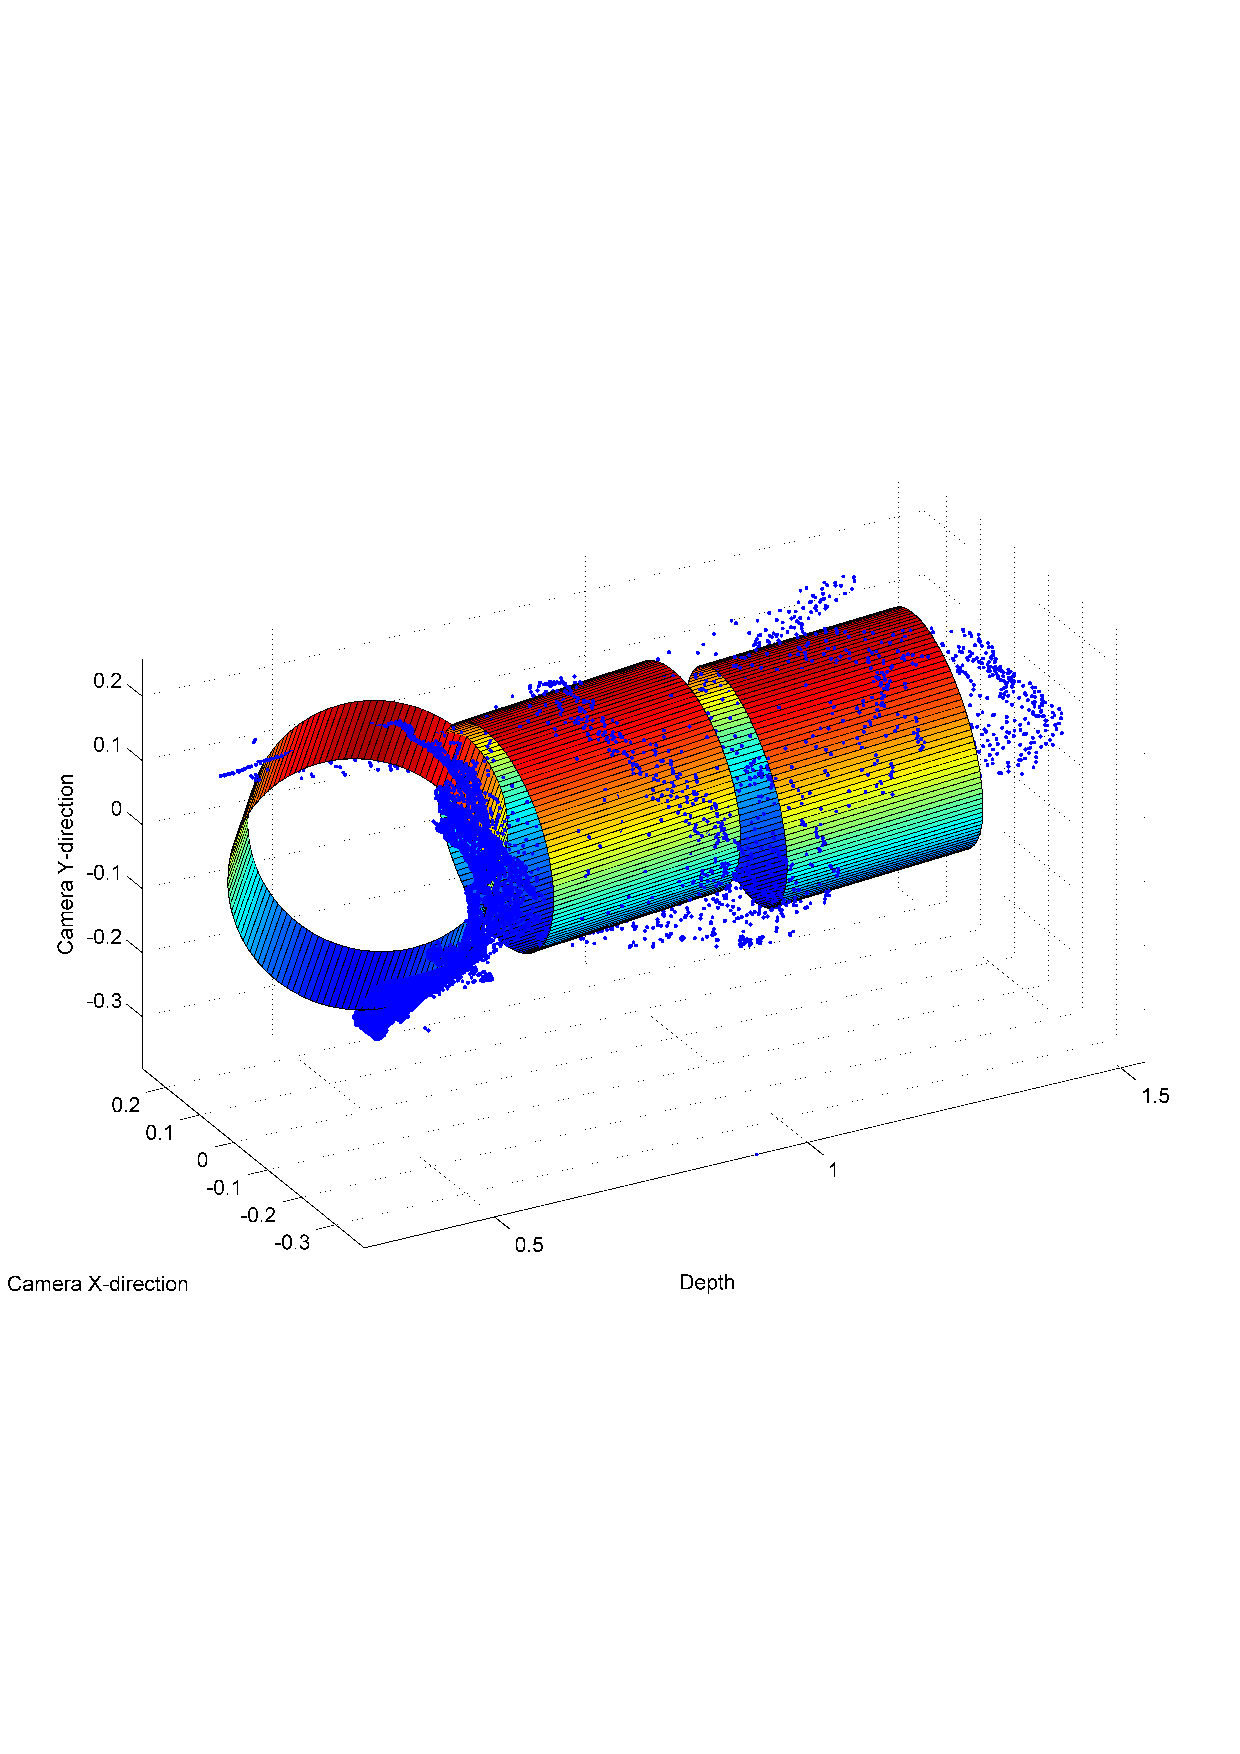
\includegraphics[width=0.8\textwidth]{pics/longpipe-tof-3d}
    \caption{The point cloud and fitted cylinders taken from the time-of-flight camera}
    \label{chap7:fig-longpipe-tof-3d}
\end{figure}
\begin{figure}[htbp]
    \centering
    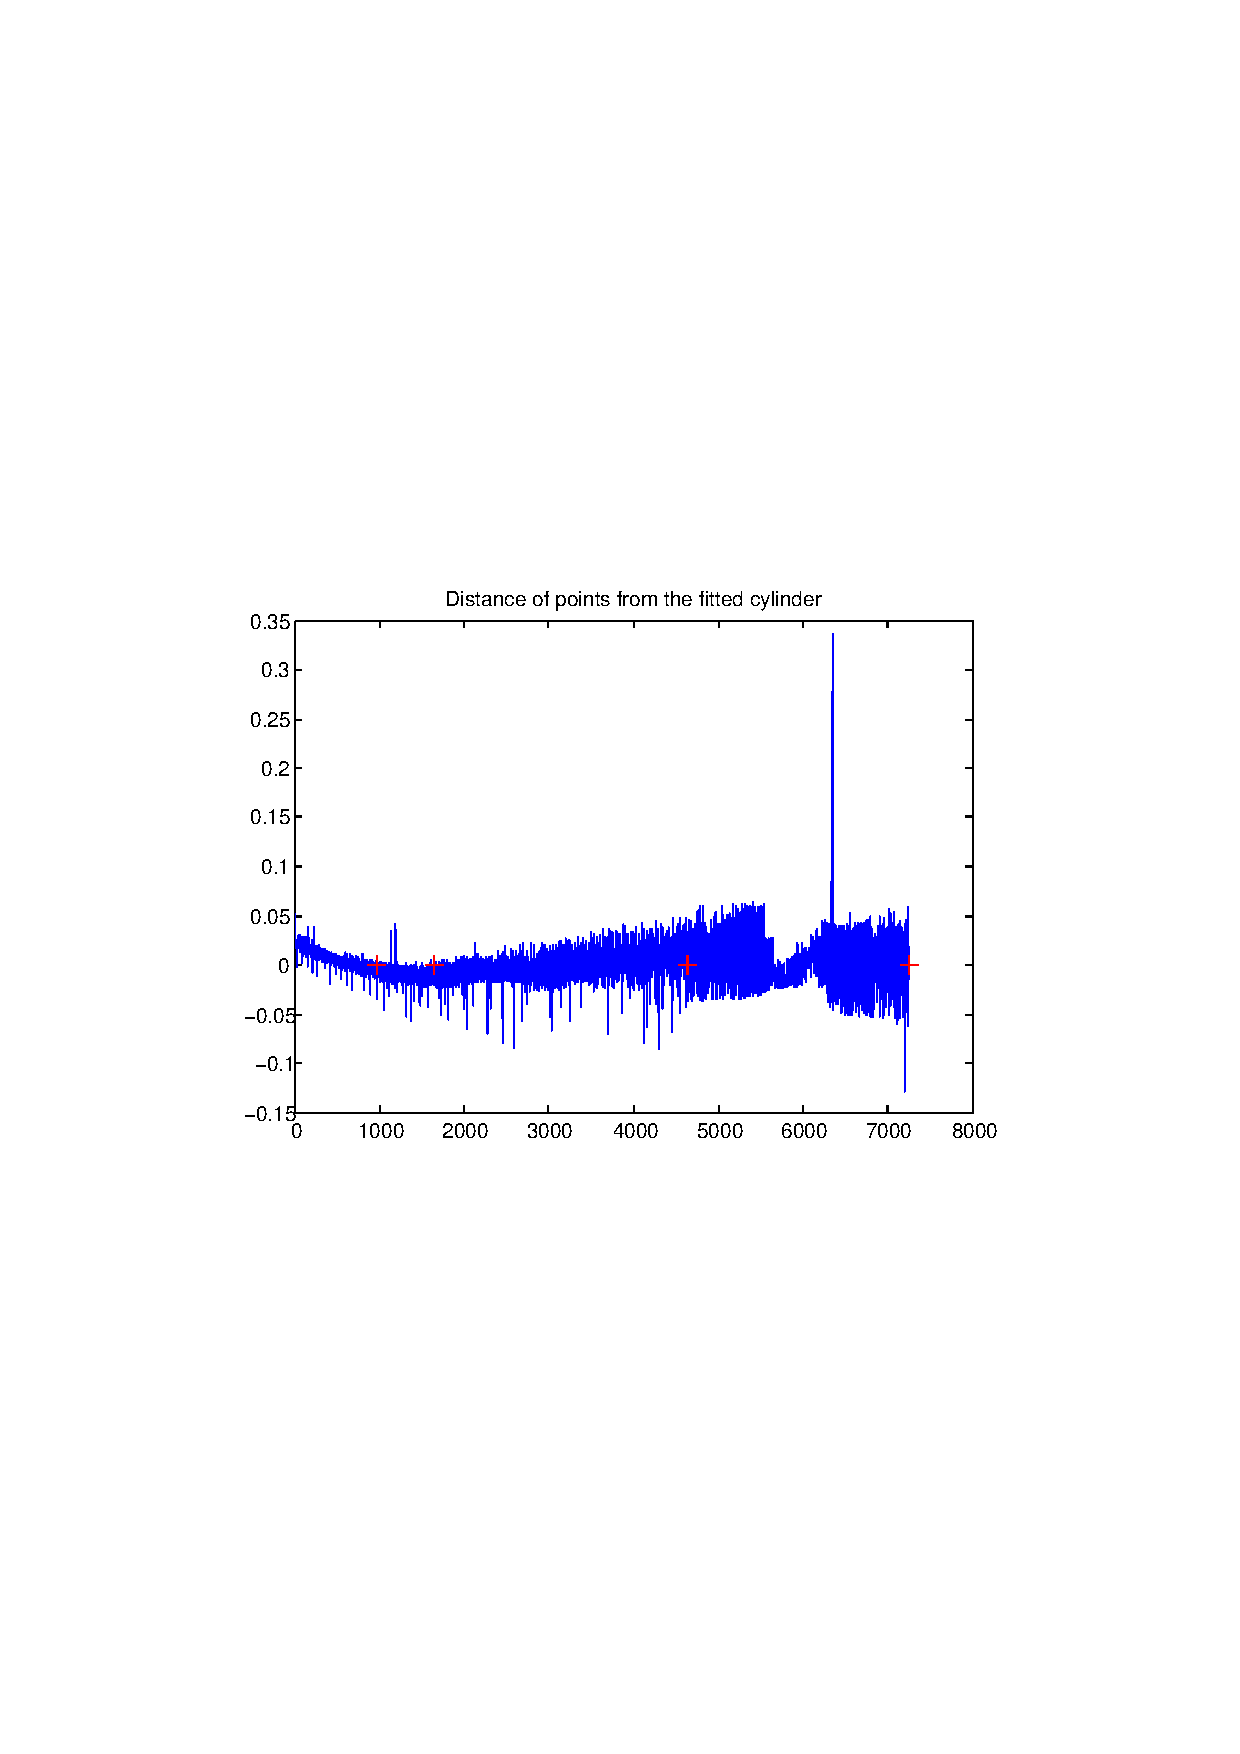
\includegraphics[width=0.8\textwidth]{pics/longpipe-tof-dist}
    \caption{The distance of the points from the fitted cylinders}
    \label{chap7:fig-longpipe-tof-dits}
\end{figure}
\begin{figure}[htbp]
    \centering
    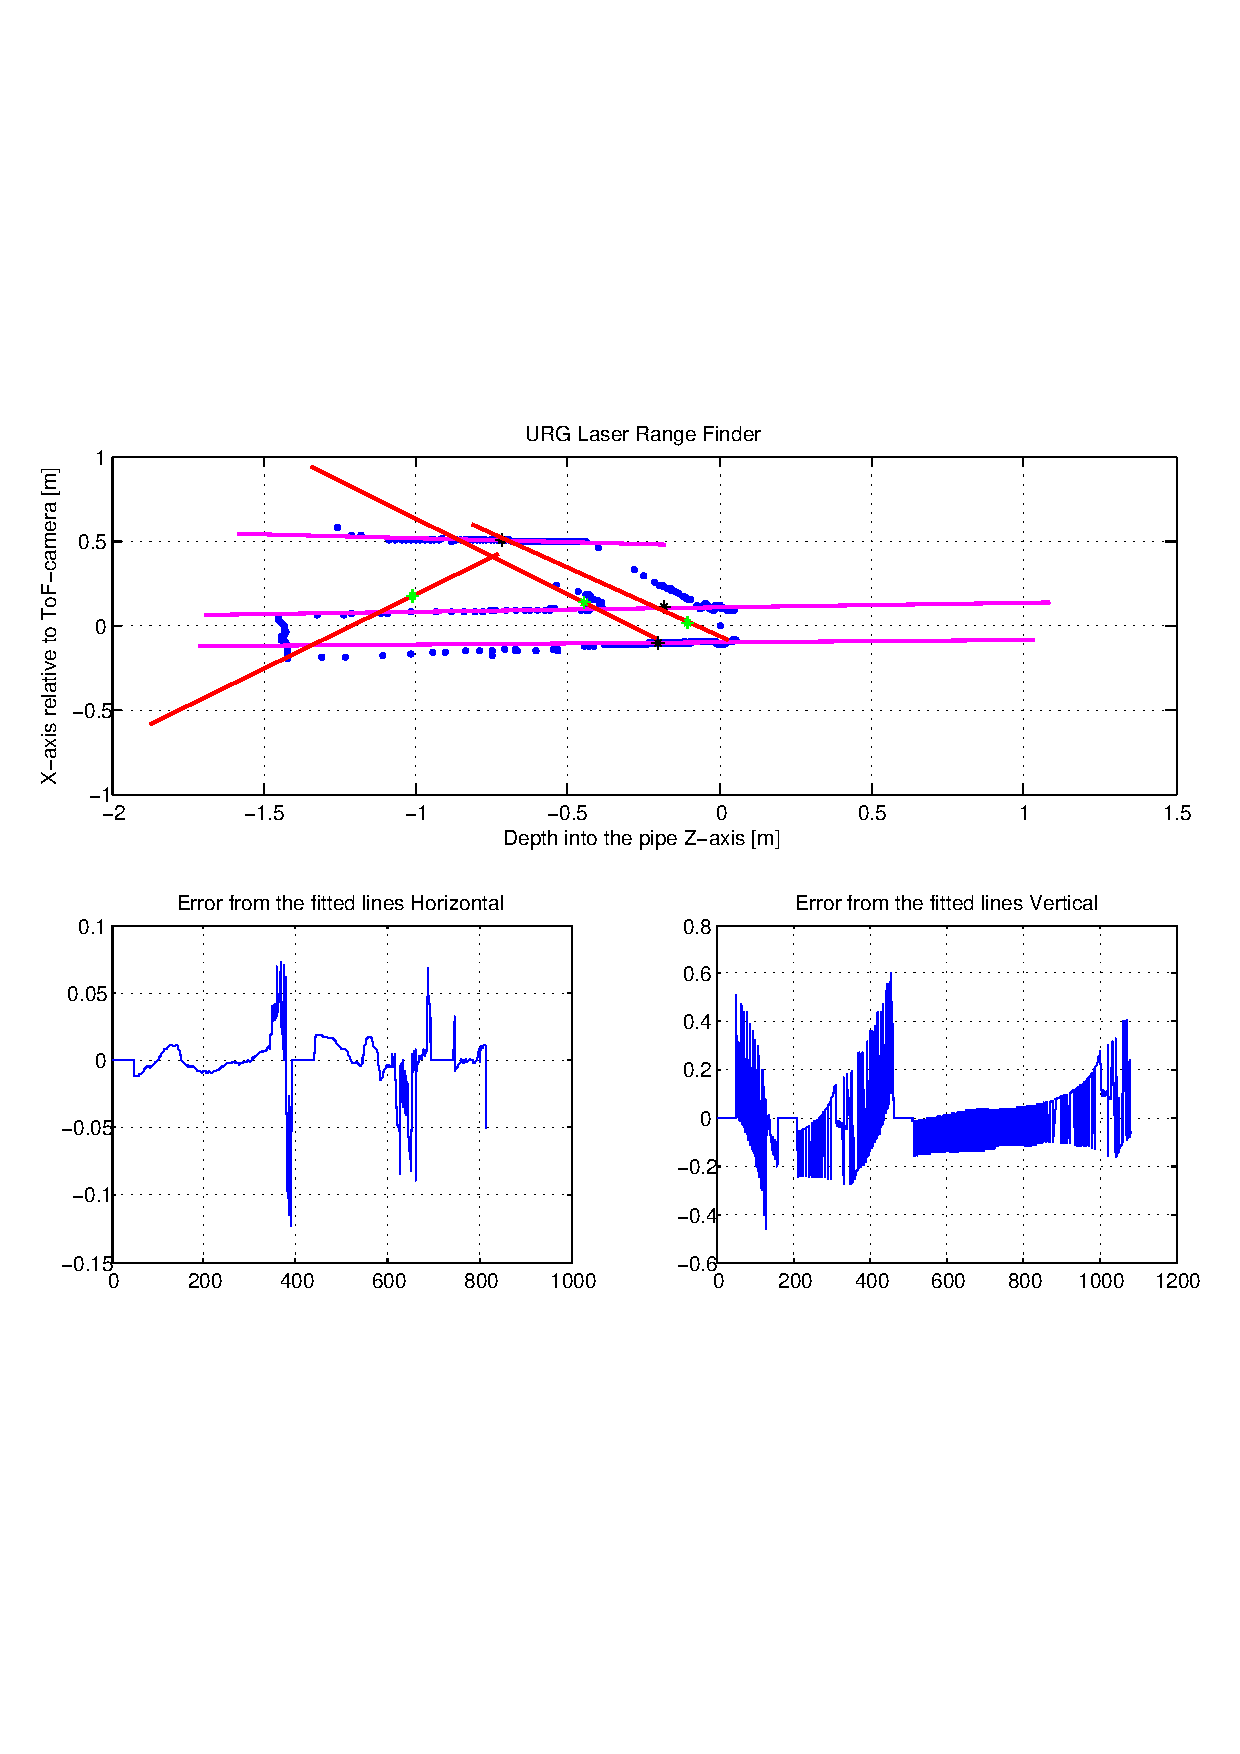
\includegraphics[width=0.8\textwidth]{pics/longpipe-urg-2d}
    \caption{The data from the URG Laser Range Finder with fitted lines}
    \label{chap7:fig-longpipe-urg-2d}
\end{figure}

\subsection{Control Case at Position Two Looking at Position One}
This this test shows how the algorithms preforms in the ideal case when placed inside the
pipe. The parameters where mostly the same as for the long pipe test.

\begin{figure}[htbp]
    \centering
    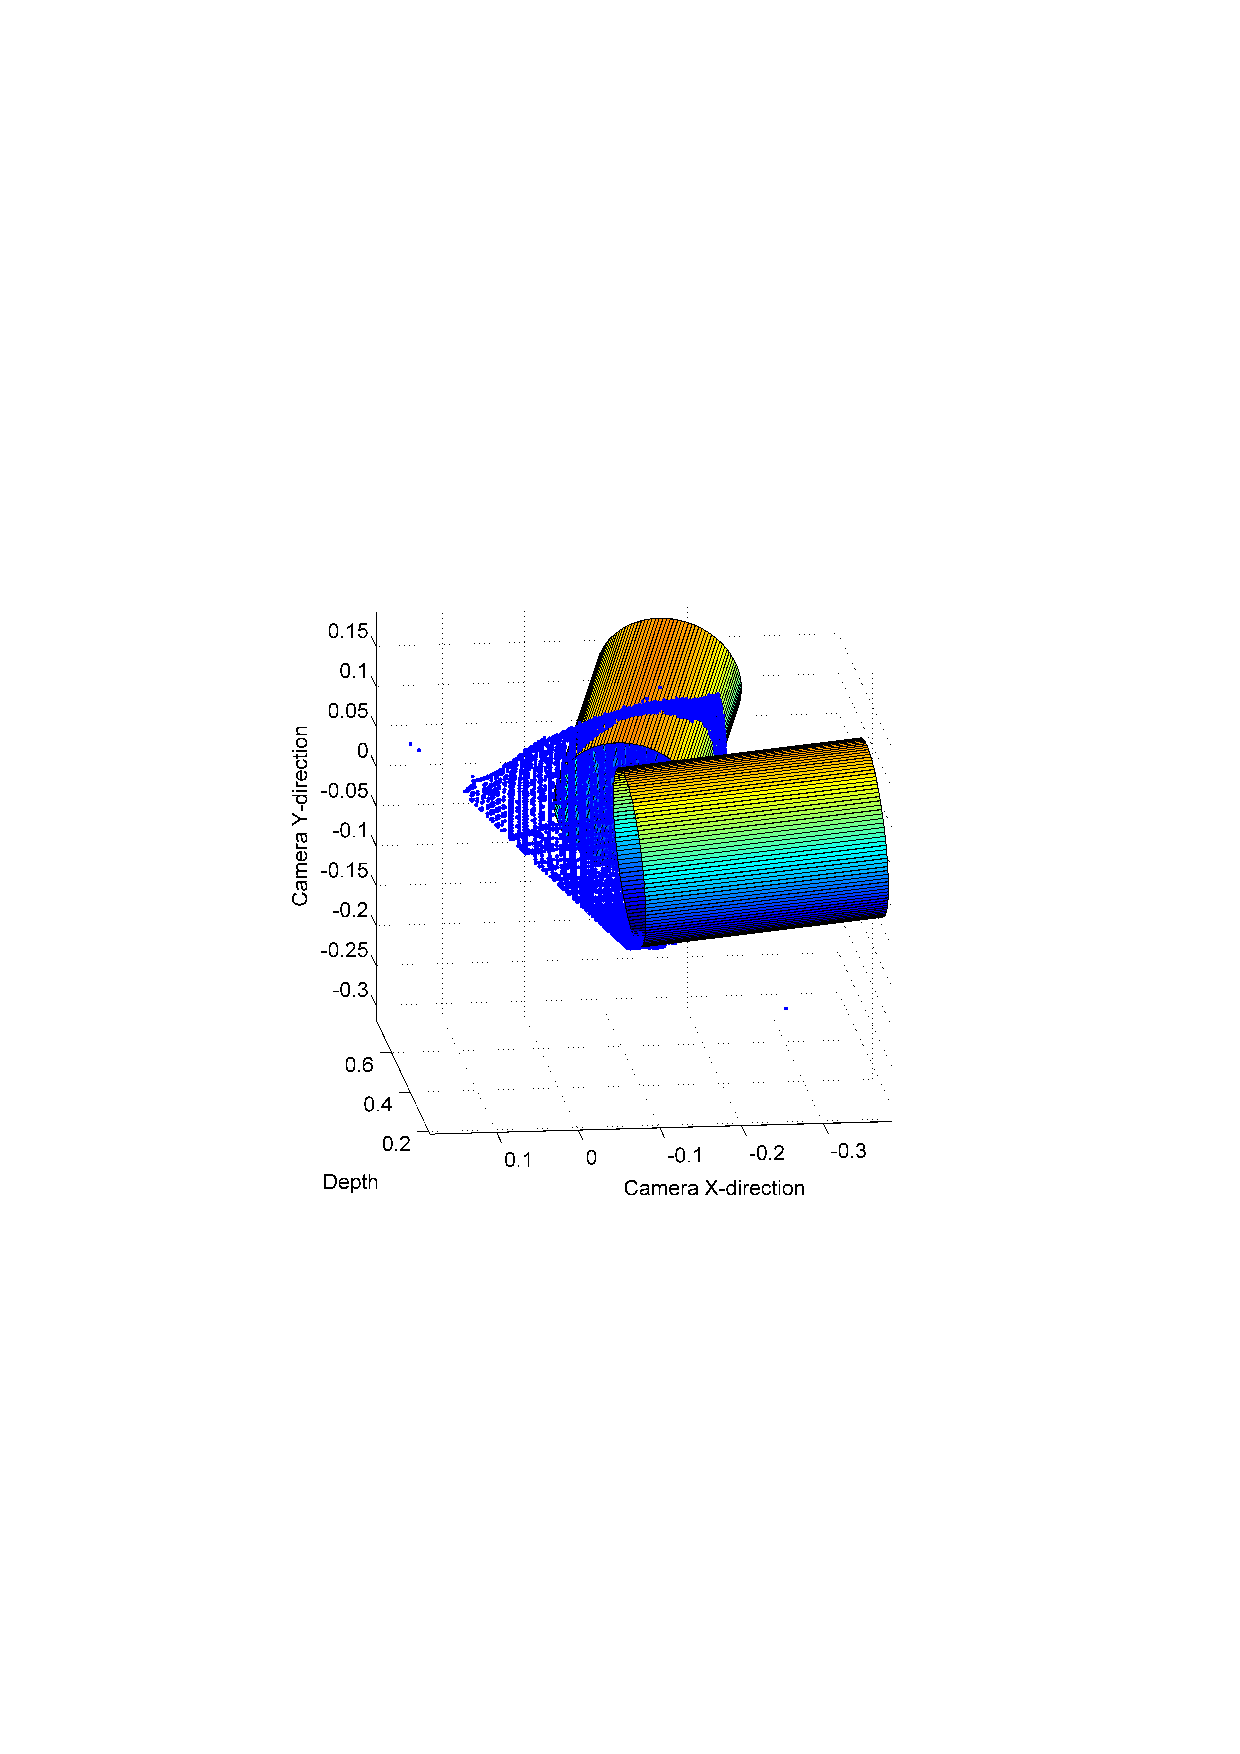
\includegraphics[width=0.8\textwidth]{pics/pos21-control-tof-3d}
    \caption{The point cloud and fitted cylinders taken from the time-of-flight camera at
    position 2}
    \label{chap7:fig-pos21-control-tof-3d}
\end{figure}
\begin{figure}[htbp]
    \centering
    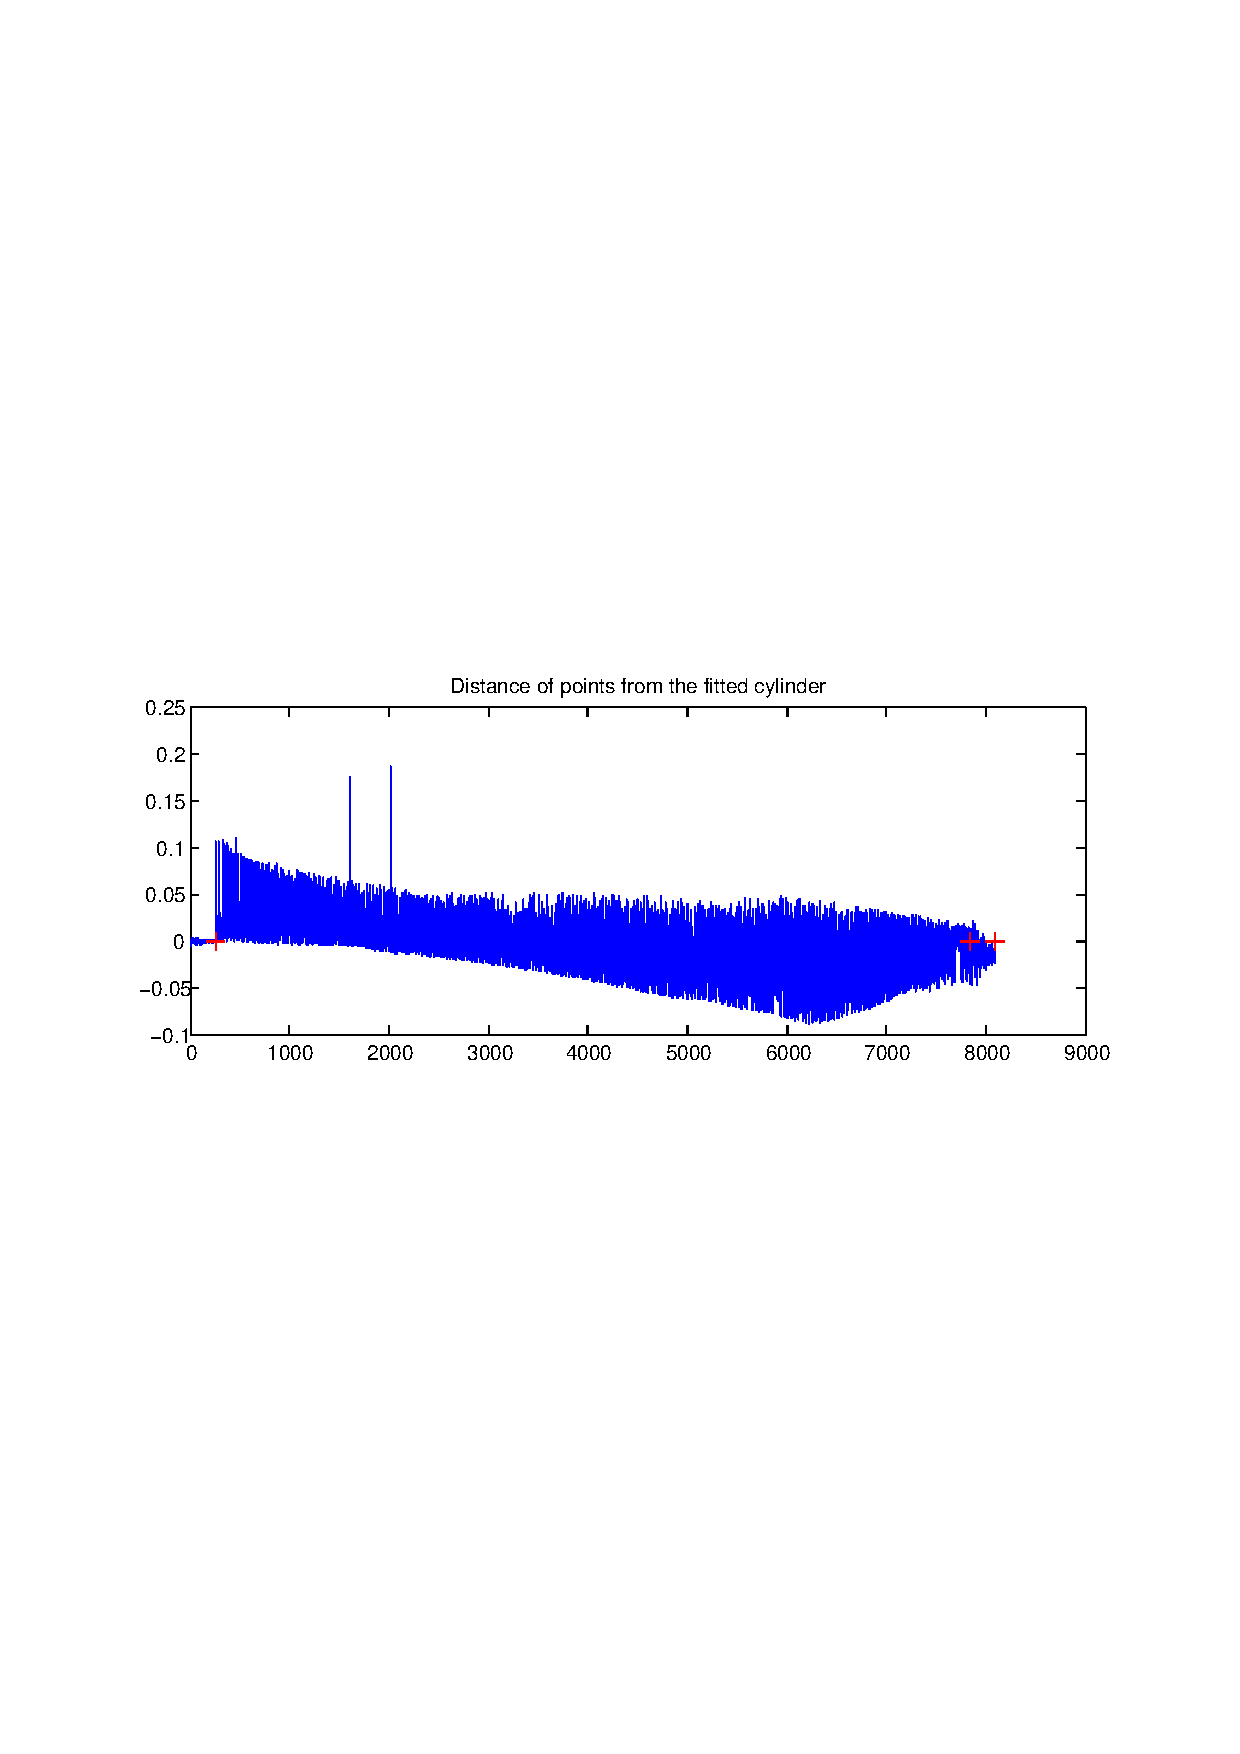
\includegraphics[width=0.8\textwidth]{pics/pos21-control-tof-dist}
    \caption{The distance of the points from the fitted cylinders at position 2}
    \label{chap7:fig-pos21-control-tof-dits}
\end{figure}
\begin{figure}[htbp]
    \centering
    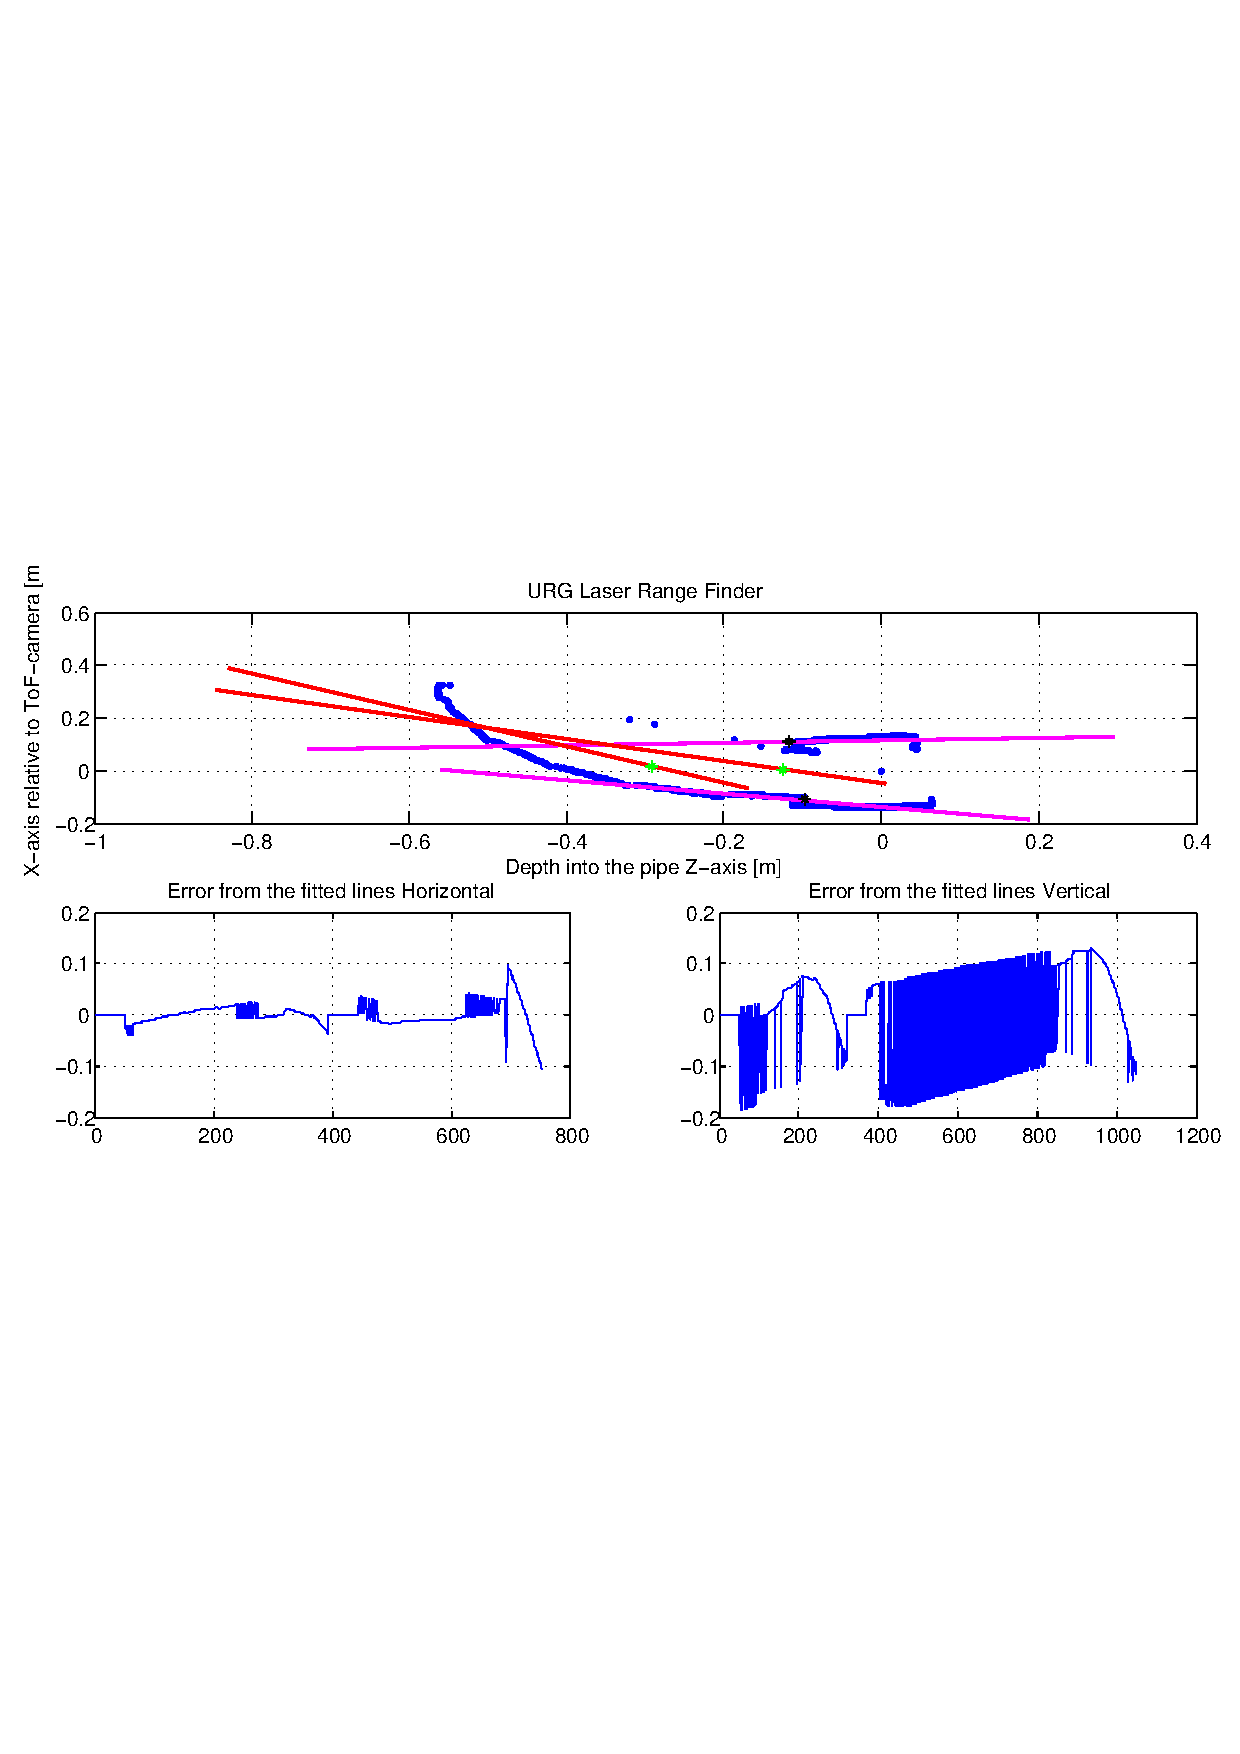
\includegraphics[width=0.8\textwidth]{pics/pos21-control-urg-2d}
    \caption{The data from the URG Laser Range Finder with fitted lines at position 2}
    \label{chap7:fig-pos21-control-urg-2d}
\end{figure}


\subsection{Irregular Obstacle at Point B at Position One}

\begin{figure}[htbp]
    \centering
    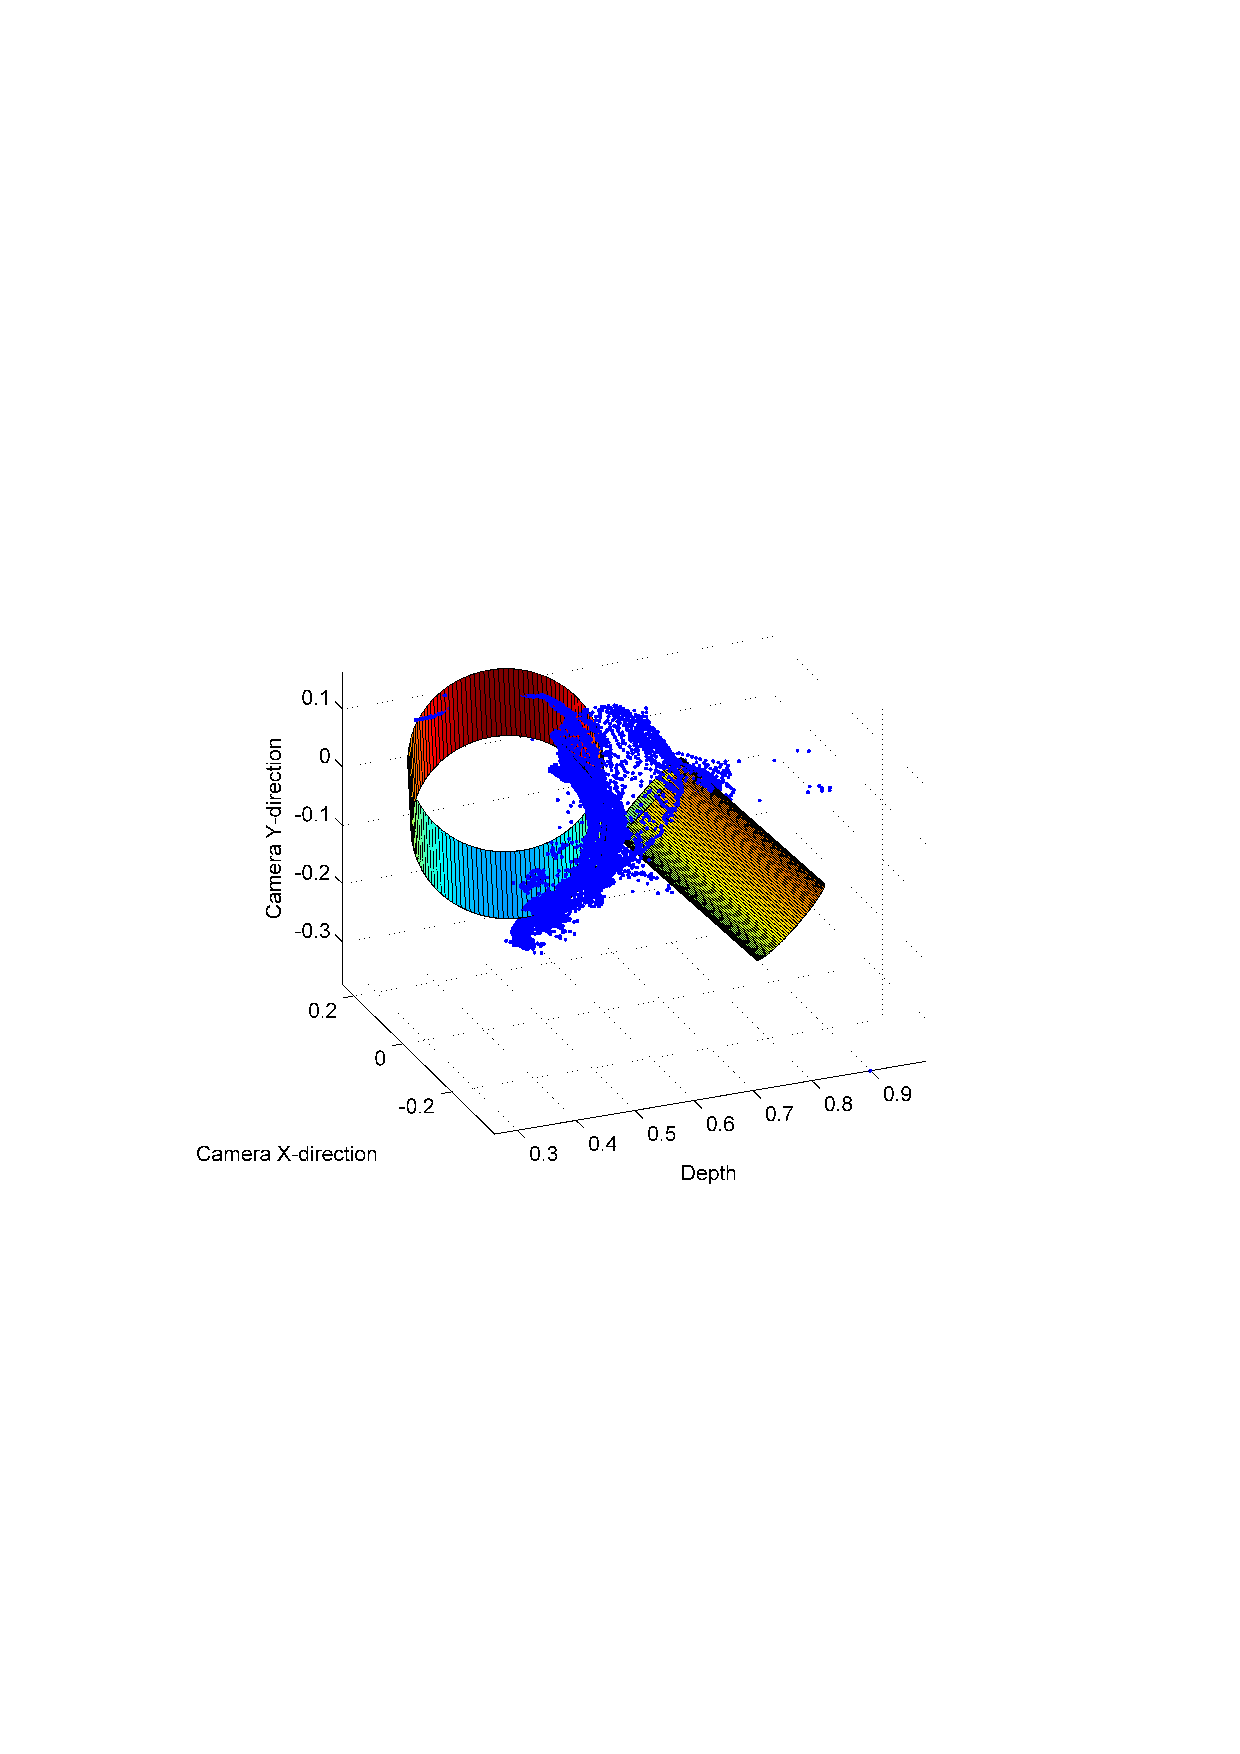
\includegraphics[width=0.8\textwidth]{pics/pos1-irregular-tof-3d}
    \caption{Fitted cylinders from ToF camera at position 1 with irregular obstacle}
    \label{chap7:fig-pos1-irregular-tof-3d}
\end{figure}
\begin{figure}[htbp]
    \centering
    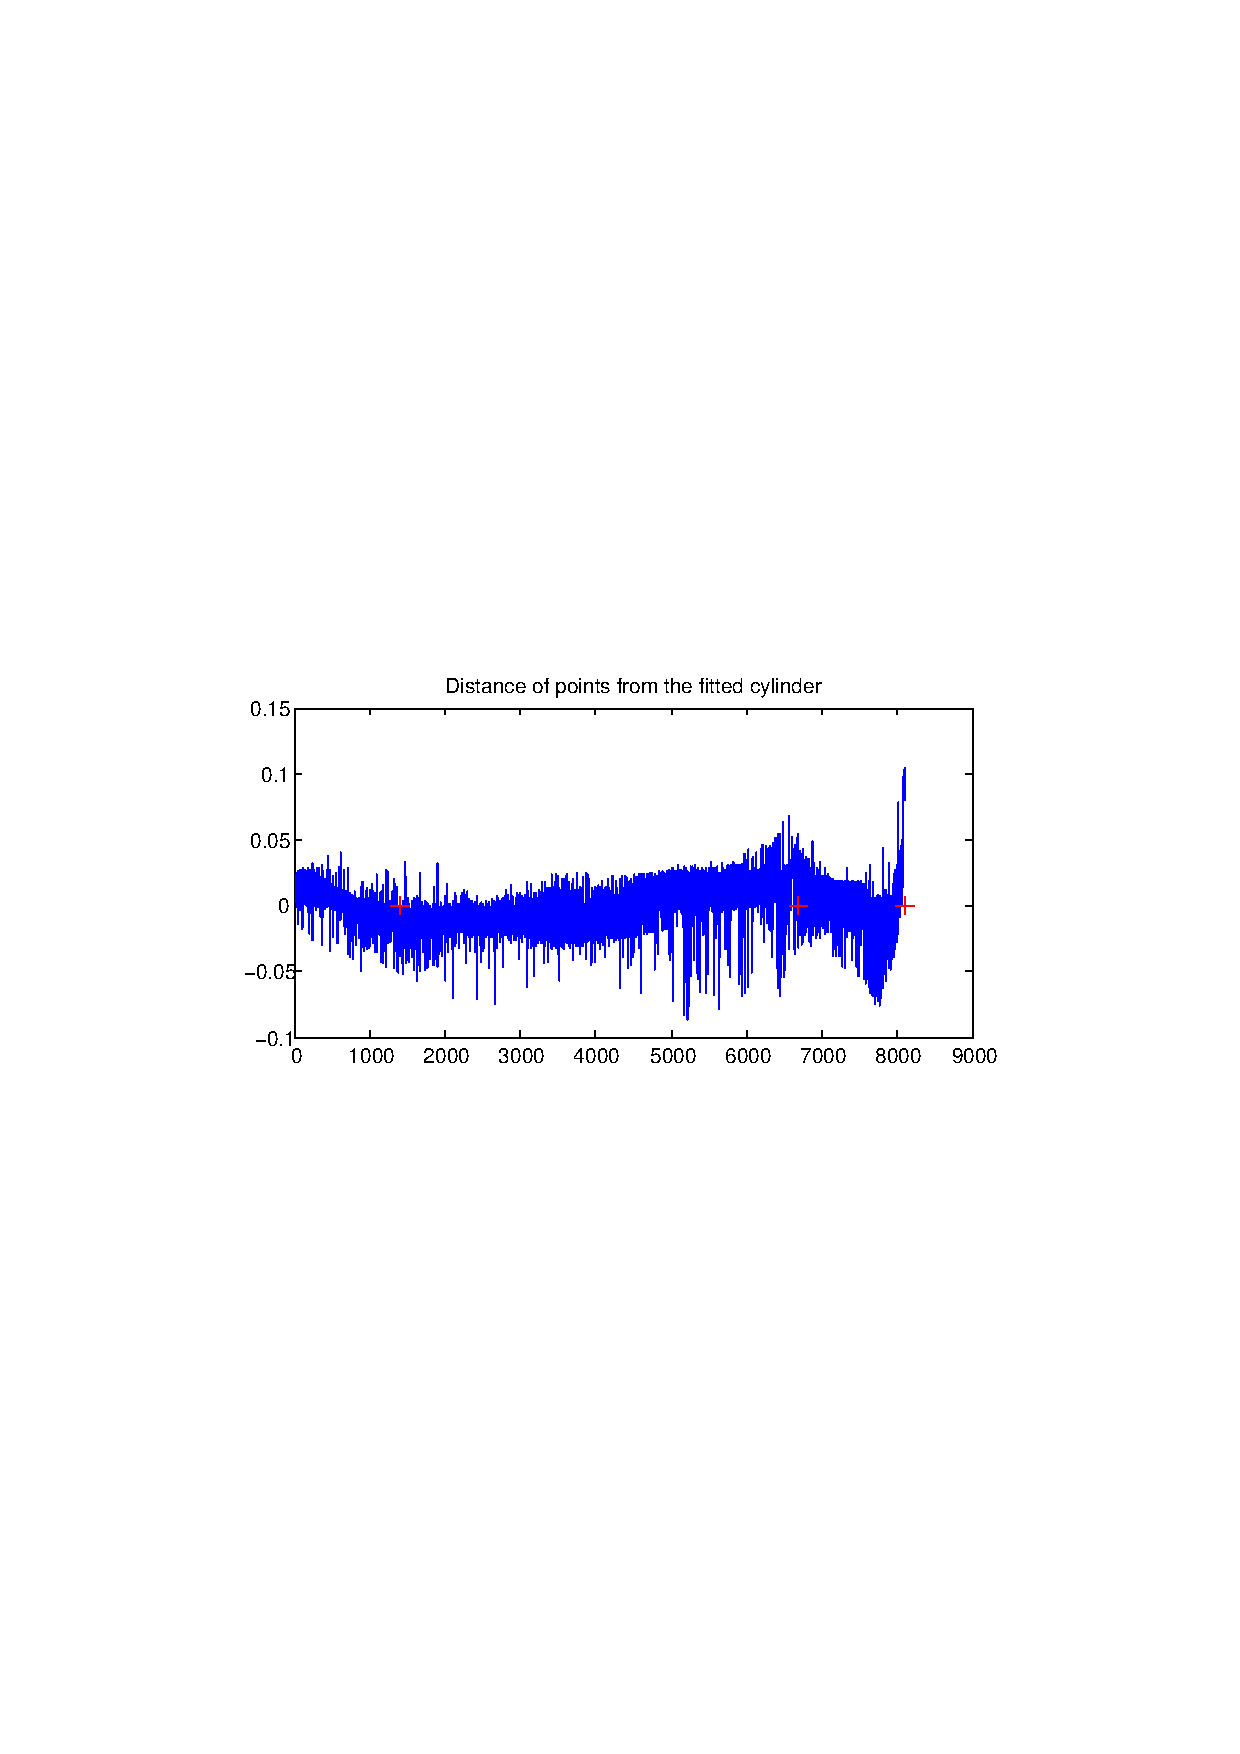
\includegraphics[width=0.8\textwidth]{pics/pos1-irregular-tof-dist}
    \caption{The distance from the fitted cylinder with irregular obstacle}
    \label{chap7:fig-pos1-irregular-tof-dits}
\end{figure}
\begin{figure}[htbp]
    \centering
    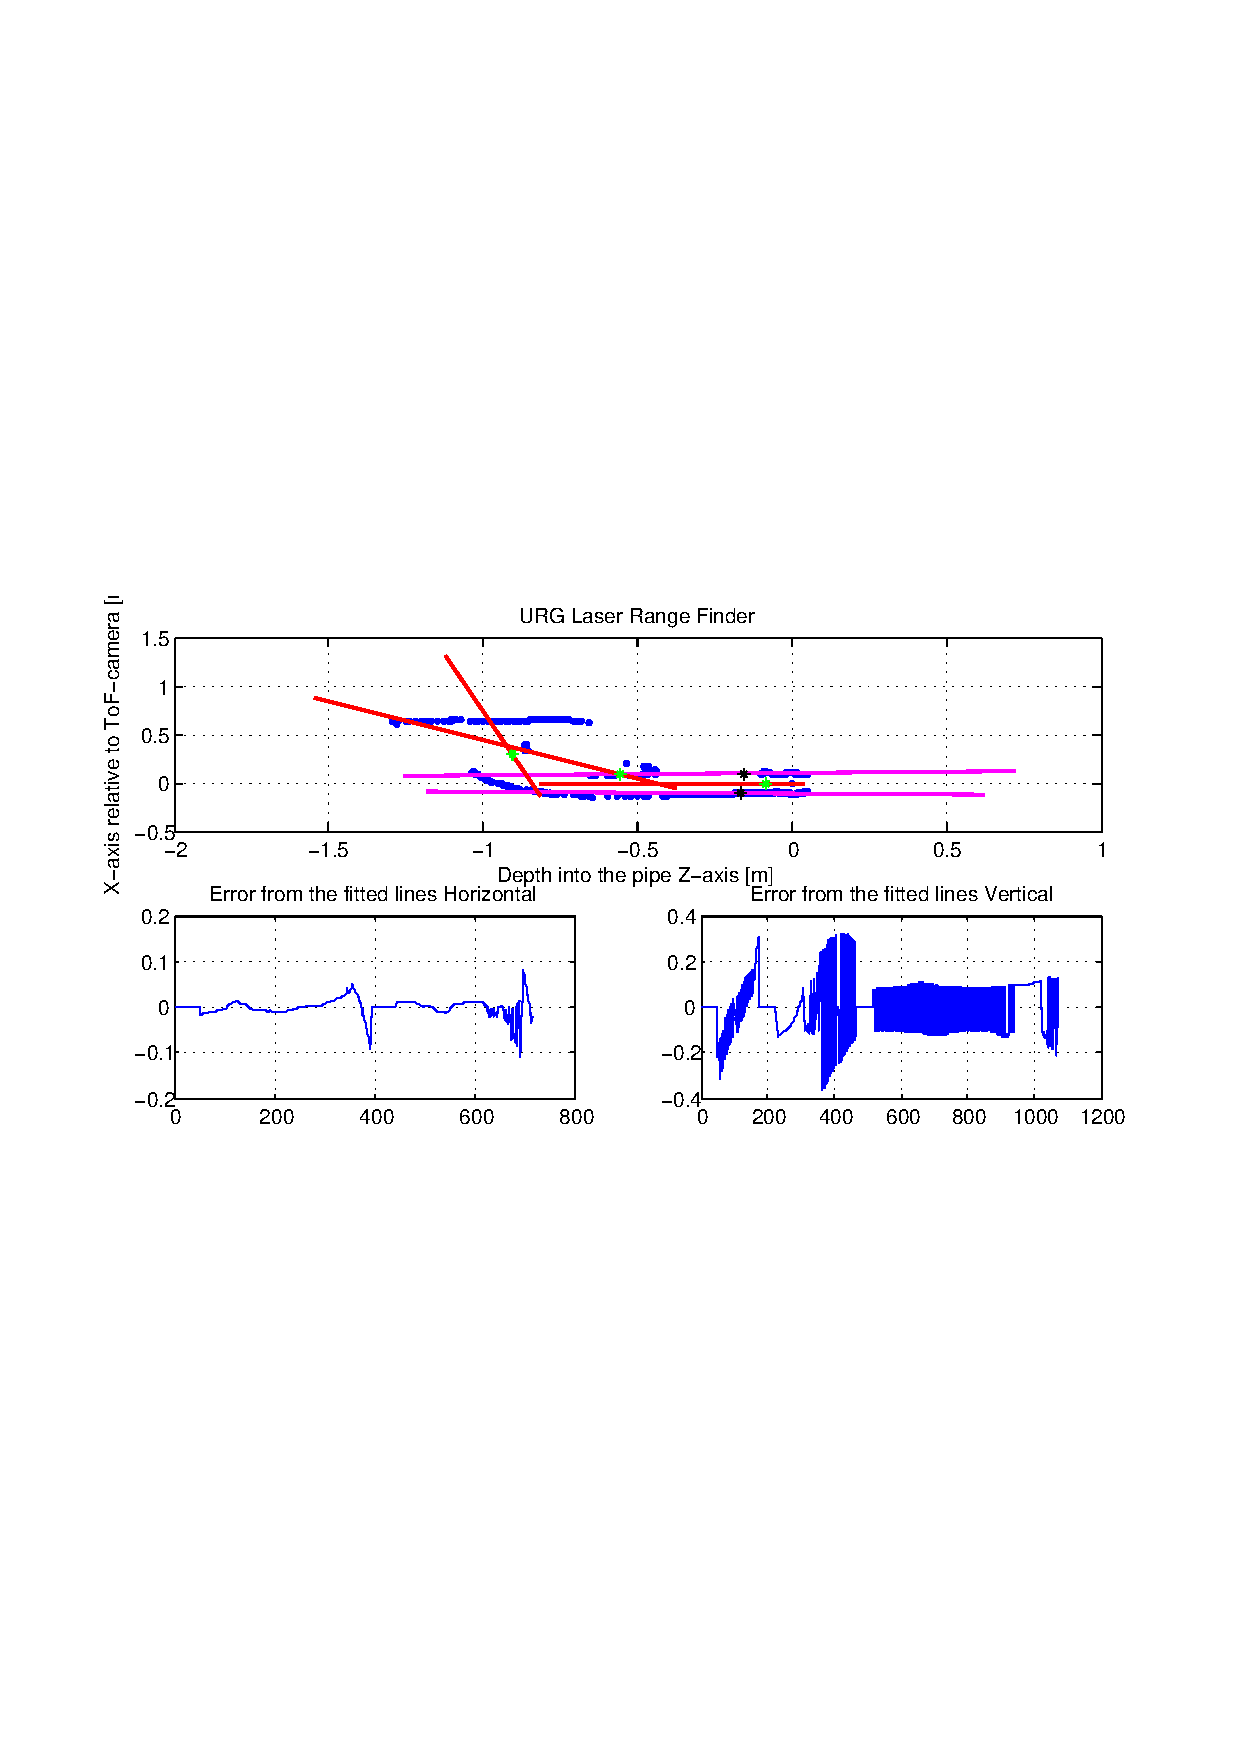
\includegraphics[width=0.8\textwidth]{pics/pos1-irregular-urg-2d}
    \caption{The data from the URG Laser Range Finder at Position 1}
    \label{chap7:fig-pos1-irregular-urg-2d}
\end{figure}
